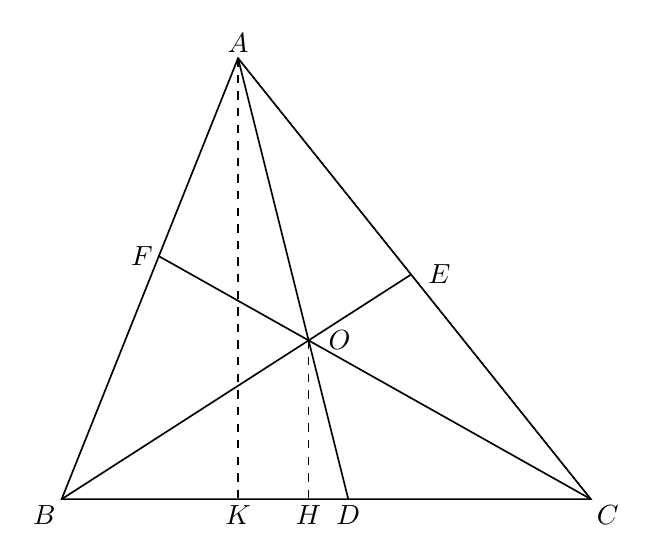
\begin{tikzpicture}[x=1cm,y=1cm,font=\normalsize,
 geometry edge/.style={solid,line width=.6pt},
 geometry mark/.style={solid,line width=.6pt},
 geometry label/.style={font=\normalsize,inner sep=2pt}]
\coordinate (A) at (2.240000000,5.600000000);
\coordinate (B) at (0.000000000,0.000000000);
\coordinate (C) at (6.720000000,0.000000000);
\coordinate (O) at (3.136000000,2.016000000);
\coordinate (D) at (3.640000000,0.000000000);
\coordinate (E) at (4.437735849,2.852830189);
\coordinate (F) at (1.234285714,3.085714286);
\coordinate (K) at (2.240000000,0.000000000);
\coordinate (H) at (3.136000000,0.000000000);
\draw[geometry edge] (A)--(B)--(C)--cycle;
\draw[geometry edge] (A)--(O);
\draw[geometry edge] (O)--(D);
\draw[geometry edge] (B)--(O);
\draw[geometry edge] (O)--(E);
\draw[geometry edge] (C)--(O);
\draw[geometry edge] (O)--(F);
\draw[geometry edge,dashed] (A)--(K);
\draw[geometry edge,dashed] (O)--(H);
\node[geometry label,above] at (A) {$A$};
\node[geometry label,below left] at (B) {$B$};
\node[geometry label,below right] at (C) {$C$};
\node[geometry label,right,xshift=5pt] at (O) {$O$};
\node[geometry label,below] at (D) {$D$};
\node[geometry label,right,xshift=4pt] at (E) {$E$};
\node[geometry label,left] at (F) {$F$};
\node[geometry label,below] at (K) {$K$};
\node[geometry label,below] at (H) {$H$};
\end{tikzpicture}